\section{Discussion}
\label{sec:discussion}

\begin{table}[b]
\centering
\caption{We report the predicted optimal vocabulary parameters $N_v$ and the vocabulary size $V$ by the proposed three approaches given $N_{nv}$. We assume the training FLOPs are optimally allocated i.e. that the non-vocabulary parameters and training data are scaled equally. ``App'' denotes the approach.}
\vspace{2mm}
\scalebox{0.85}{
\setlength{\tabcolsep}{1.5mm}{
\begin{tabular}{c|ccc|c|ccc|c}
\toprule
\textbf{$N_{\rm nv}$} & \textbf{$N_{\rm v}^{\rm opt}$-App1} & \textbf{$N_{\rm v}^{\rm opt}$-App2}  & \textbf{$N_{\rm v}^{\rm opt}$-App3} & \textbf{Dim.}  & \textbf{$V^{\rm opt}$-App1}  & \textbf{$V^{\rm opt}$-App2} & \textbf{$V^{\rm opt}$-App3}  & \textbf{FLOPs Budget} \\
\midrule
% 1B           & 0.1B                    & 0.1B                  & 2048       & 29K                & 25K               &  0.1T      \\ 
3B           &           0.1B      &  0.1B    & 0.1B                 & 3200       &  39K                & 43K   &     37K            &  $1.3e21$ \\ 
7B           & 0.3B&   0.3B   &  0.2B                         & 4096       &     62K           &67K    &    60K           & $7.1e21$  \\ 
13B          &0.4B&0.5B  &   0.4B           & 5120       &   83K    &91K              & 81K               & $2.4e22$    \\
30B          &       0.9B             & 0.9B & 0.9B              & 6048       &     142K            &      154K           & 142K & $1.3e23$    \\ 
70B          &           1.7B         &1.9B &1.8B                  & 8192       &     212K    &    231K      &218K                & $7.1e23$  \\
130B         &      2.9B             &  3.2B &3.0B                  & 12888      &      237K           & 258K  &248K                & $2.4e24$  \\
300B         &   5.8B      &     6.4B      &6.3B                 & 16384      &356K &389K                  &       383K          & $1.3e25$ \\ 
\bottomrule
\end{tabular}
}}

\label{tab:predict}
\end{table}

\paragraph{Predicting allocations for larger models}

\autoref{tab:predict} reports the predicted optimal vocabulary parameters and sizes based on the proposed three approaches, where the amount of training data is optimally allocated, \textit{i.e.} equally scaled with the non-vocabulary parameters~\citep{hoffmann2022training}. Aligned with the trend shown in \autoref{fig:intro}, \textit{the predictions from all proposed approaches align closely}. $N_{\rm nv}$ should be scaled faster than $N_{\rm v}$. Notably, mainstream LLMs typically assign fewer parameters to vocabulary than what is optimal. However, the community is starting to shift to larger vocabularies, such as with Llama3~\cite{metallama3blog} having a 128K vocabulary size up from 32K of Llama2~\citep{touvron2023llama}. However, scaling data is still the most critical part, and solving data scarcity issues should be a focus of future work~\citep{villalobos2022will}.

\begin{table}[t]
\centering
\small
\caption{Zero-shot performance of models with $N_{nv}=2.87B$ comparing the commonly used $V=32K$ with our predicted optimal vocabulary $V^{opt}$. We consider the scenario where the number of training data is equally scaled with the non-vocabulary parameters. We report accuracy and standard deviation in percentages. Accuracy is normalized: The predicted likelihoods are divided by the length of each choice for multiple choices to eliminate the effect of text length on predictions.}
\vspace{1mm}
\scalebox{0.95}{
\setlength{\tabcolsep}{0.8mm}{
\begin{tabular}{cccc|ccccccc|c}
\toprule
&\textbf{$N_{\rm v}$}& \textbf{$D$} &\textbf{$H$}& \textbf{ARC-C} & \textbf{ARC-E} & \textbf{Hellaswag} & \textbf{OBQA} & \textbf{WG} & \textbf{PIQA} & \textbf{BoolQ} &\textbf{Average}\\
\midrule
\multicolumn{12}{c}{\textit{FLOPs Budget 1.2e21 (Optimally-Allocated Training Data)}}
\vspace{1mm}
\\
% \dashline
$V$=32K  & 0.10B&67.3B & 266.6B&
{28.5}{\tiny $\pm$1.3} & {49.2}{\tiny $\pm$1.0} & {47.5}{\tiny $\pm$0.5} & {31.6}{\tiny $\pm$2.1} & {50.4}{\tiny $\pm$1.4} & {71.4}{\tiny $\pm$1.1} & {56.4}{\tiny $\pm$0.9}&47.9
\\
$V^{opt}$=35K&0.11B & 67.1B& 268.2B&
\textbf{29.1}{\tiny $\pm$1.3} & \textbf{50.6}{\tiny $\pm$1.0} & \textbf{48.1}{\tiny $\pm$0.5} & \textbf{31.6}{\tiny $\pm$2.1} & \textbf{51.9}{\tiny $\pm$1.4} & \textbf{71.4}{\tiny $\pm$1.1} & \textbf{57.1}{\tiny $\pm$0.9}&\textbf{48.5}
\\
\bottomrule
\end{tabular}
}}
\label{tab:downstream-3Bmodel-optimal}
\end{table}

To empirically verify our prediction, we train models with $N_{\rm nv}=2.87B$ under a compute-optimal training FLOPs budget and evaluate them using lighteval~\footnote{\url{https://github.com/huggingface/lighteval}}. For the baseline model we use the common vocabulary size of $V=32K$. The other model uses $V^{\rm opt}$ as predicted by Approach 3. In \autoref{tab:downstream-3Bmodel-optimal}, we show that the model allocated according to our vocabulary predictions yields better performance across multiple downstream tasks. This verifies that our predictions hold at scale.



\paragraph{Experiments with scarce and excessive training data} Our prior experiments focus on the setting where training compute budget is the main constraint and we seek to allocate it optimally to parameters and training data. This is the typical setting in scaling law studies~\citep{kaplan2020scaling,hoffmann2022training,rae2021scaling}. However, in the real world, we often deal with scarce data (``data-constrained~\citep{muennighoff2024scaling}'') forcing us to train sub-optimally or would like to make use of excessive data to train a smaller model that is cheaper to use \citep{zhang2024tinyllama}. To verify that our Approach 3 can handle these practical scenarios, we compare the model with $V=32K$ and the model with the vocabulary size $V^{\rm opt}$ predicted by Approach 3. As shown in Table \ref{tab:downstream-3Bmodel}, our prediction enables a better model by only adjusting the vocabulary size in different FLOPs budgets.


\begin{table}[t]
\centering
\small
\caption{Zero-shot performance of models with $N_{\rm nv}\!=\!2.87B$ comparing the commonly used $V=32K$ with our predicted optimal vocabulary $V^{\rm opt}$ when \textbf{undertraining} or \textbf{overtraining}.
}
% Nv=205M (v=32k), Nv=275M(v=43k)
\vspace{1mm}
\scalebox{0.95}{
\setlength{\tabcolsep}{0.8mm}{

\begin{tabular}{cccc|ccccccc|c}
\toprule
&\textbf{$N_{\rm v}$}& \textbf{$D$} &\textbf{$H$}& \textbf{ARC-C} & \textbf{ARC-E} & \textbf{Hellaswag} & \textbf{OBQA} & \textbf{WG} & \textbf{PIQA} & \textbf{BoolQ} &\textbf{Average}\\
\midrule
\multicolumn{12}{c}{\textit{FLOPs Budget 2.8e20 (Insufficient Training Data, ``Undertraining'')}}
\vspace{1mm}
\\
$V$=32K &0.10B &15.7B &62.2B & 
{23.6}{\tiny $\pm$1.2} & {40.8}{\tiny $\pm$1.0} & {34.4}{\tiny $\pm$0.5} & \textbf{29.0}{\tiny $\pm$2.0} & {49.7}{\tiny $\pm$1.4} & {64.9}{\tiny $\pm$1.1} & {59.8}{\tiny $\pm$0.9}&43.2

\\
$V^{\rm opt}$=24K& 0.08B & 15.8B&60.8B & 
\textbf{24.2}{\tiny $\pm$1.3} & \textbf{42.2}{\tiny $\pm$1.0} & \textbf{36.0}{\tiny $\pm$0.5} & {28.6}{\tiny $\pm$2.0} & \textbf{50.0}{\tiny $\pm$1.4} & \textbf{64.9}{\tiny $\pm$1.1} & \textbf{61.5}{\tiny $\pm$0.9}&\textbf{43.9}
\\
\midrule

\multicolumn{12}{c}{\textit{FLOPs Budget 2.3e21 (Overly Sufficient Training Data, ``Overtraining'')}}
\vspace{1mm}
\\
% \midrule
$V$=32K &0.10B&128.5B&509.1B& 
{29.1}{\tiny $\pm$1.3} & {53.5}{\tiny $\pm$1.0} & {53.0}{\tiny $\pm$0.5} & {33.0}{\tiny $\pm$2.1} & {52.0}{\tiny $\pm$1.4} & {72.0}{\tiny $\pm$1.1} & {59.5}{\tiny $\pm$0.9}&50.3

\\
% \midrule
$V^{\rm opt}$=43K&0.14B &127.0B&517.5B& 
\textbf{32.0}{\tiny $\pm$1.4} & \textbf{54.7}{\tiny $\pm$1.0} & \textbf{54.1}{\tiny $\pm$0.5} & \textbf{33.0}{\tiny $\pm$2.1} & \textbf{52.8}{\tiny $\pm$1.4} & \textbf{72.6}{\tiny $\pm$1.0} & \textbf{61.9}{\tiny $\pm$0.9}&\textbf{51.6}
\\
\bottomrule
\end{tabular}
}}
\label{tab:downstream-3Bmodel}
\end{table}

In \autoref{fig:shiftv}, we further study the trend about how does the optimal  vocabulary size shift with different number of training  data. We only vary the amount of data but keep the non-vocabulary parameters fixed. The choices of vocabulary size are $8K$, $10K$, $16K$, $24K$, $32K$ and $48K$. Taking $N_{nv}=302M$ as an example, \textbf{when available data is the bottleneck, the optimal vocabulary size decreases empirically}, \textit{i.e.} $16K \rightarrow 10K$. This is a mechanism to prevent over-fitting. Conversely, {when training on excessive amounts of data}, \textit{e.g.}, Llama3-8B uses much more training tokens than what would be compute-optimal for its budget, \textbf{the optimal vocabulary size increases}, \textit{i.e.} $16K \rightarrow 24K$. Note that here we focus solely on training compute-optimal. It is also important to note that expanding the vocabulary size also increases the computational demands during inference.
Therefore, we recommend \textbf{using the optimal vocabulary size corresponding to a given $\mathbf{N_{\rm nv}}$, assuming optimal allocation of training data}, even in scenarios where overtraining may occur.

\begin{figure}[t]
\centering
\begin{subfigure}[b]{0.48\textwidth}  
    \centering
    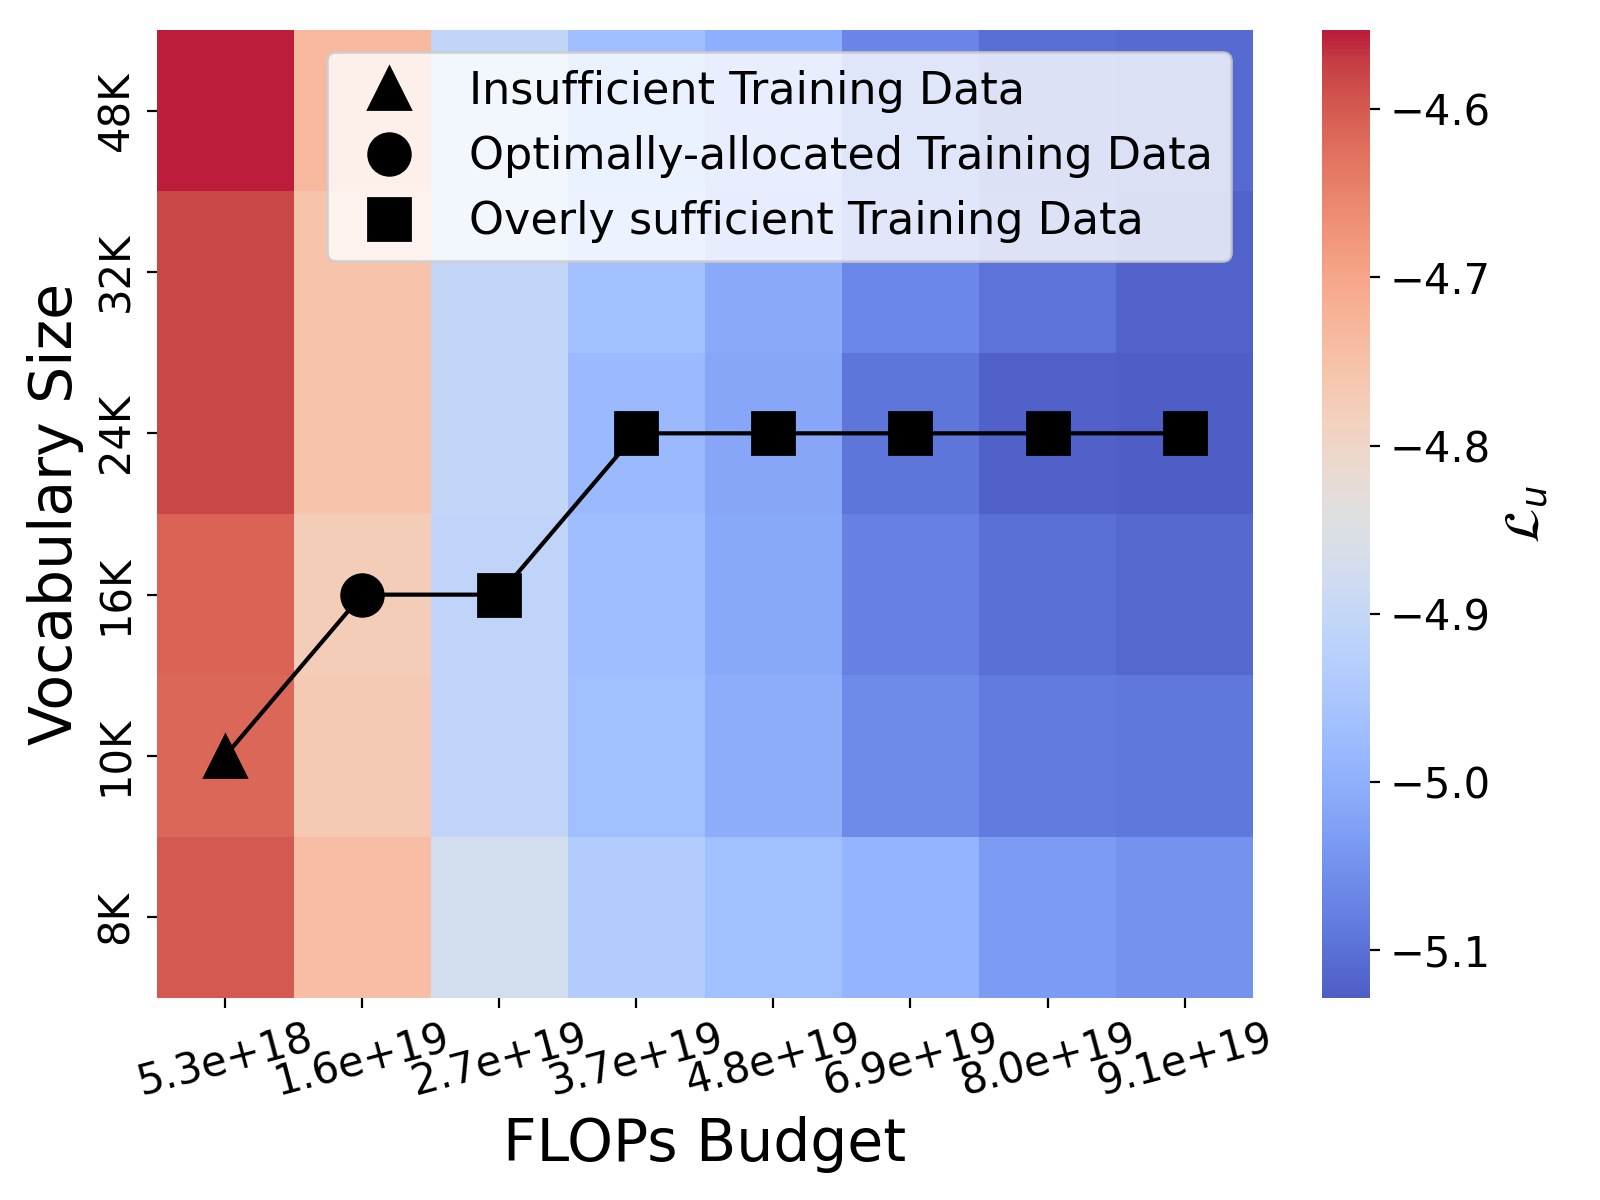
\includegraphics[width=\textwidth]{figures/matrix_335m_shiftv.png}
    % \label{fig:search_v-d}
\end{subfigure}
\begin{subfigure}[b]{0.365\textwidth} 
    \centering
    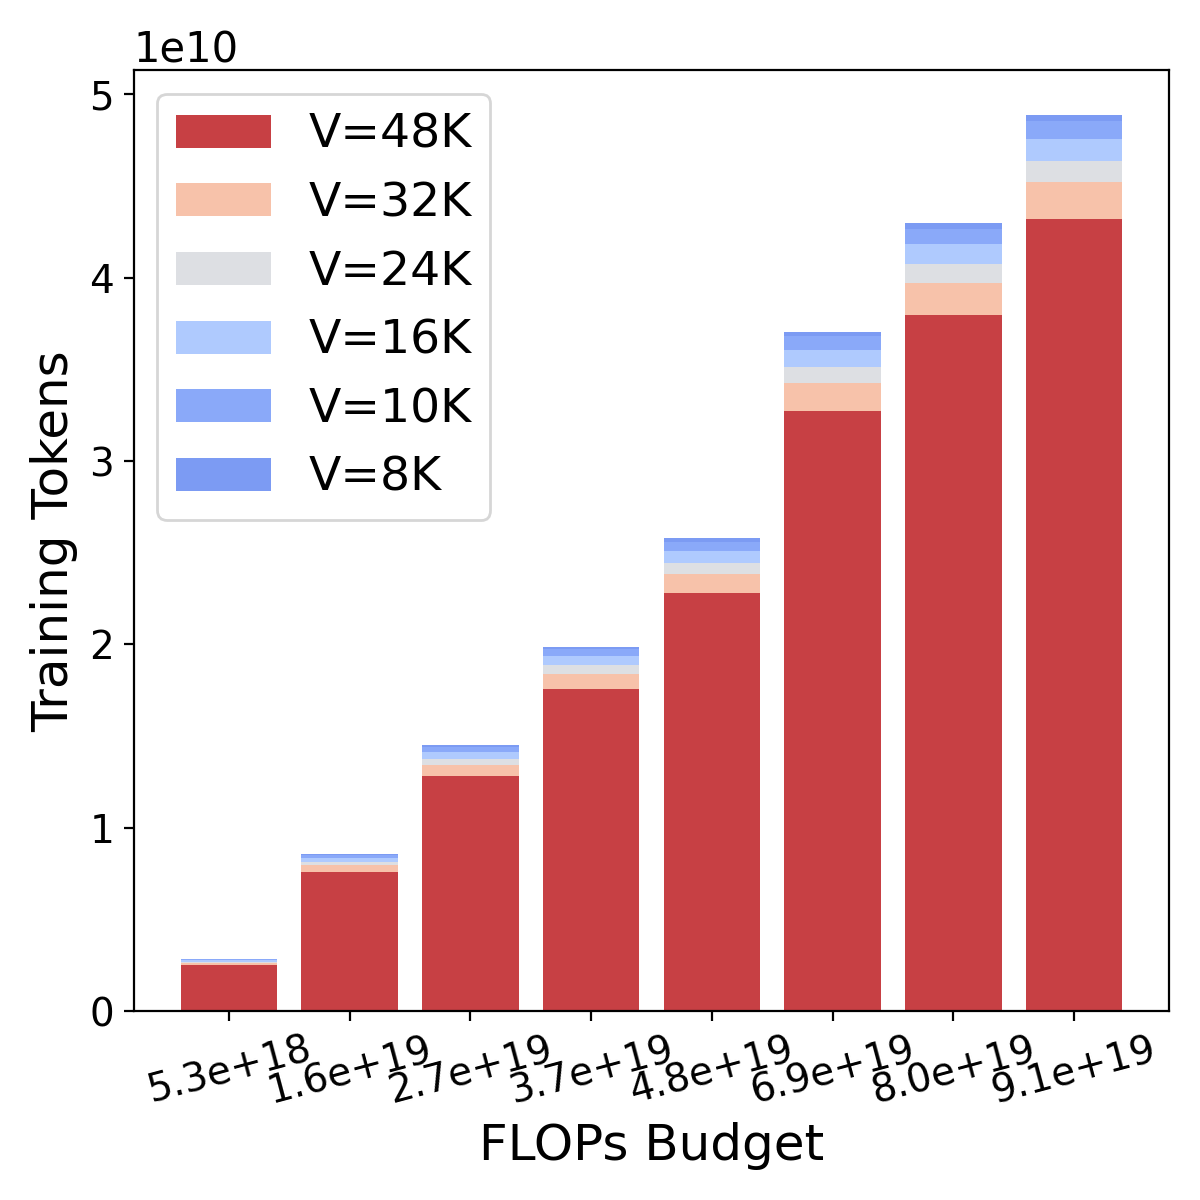
\includegraphics[width=\textwidth]{figures/matrix_335m_shiftv-new1-number-D.png}
    % \label{fig:search_Nnv_2vd}
\end{subfigure}

\caption{\textbf{Left:} The heatmap illustrates how the best vocabulary size among all choices of vocabularies shifts with the training data. The non-vocabulary parameter is fixed ($N_{nv}=302M$). Each cell in the heatmap represents the loss given a certain FLOPs budget for a fair evaluation, with the color intensity indicating the loss value. The black line with markers denotes the best vocabulary size for each FLOPs budget, which basically increases as the number of training data increases. \textbf{Right:} The number of training tokens are slightly varying for different vocabulary sizes given a certain FLOPs budget. To keep FLOPs consistent, models with larger vocabulary sizes are trained on fewer tokens.}
  \label{fig:shiftv}

\end{figure}

